\documentclass[tikz,border=3.14mm]{standalone}
\usetikzlibrary{arrows.meta, positioning}

\begin{document}

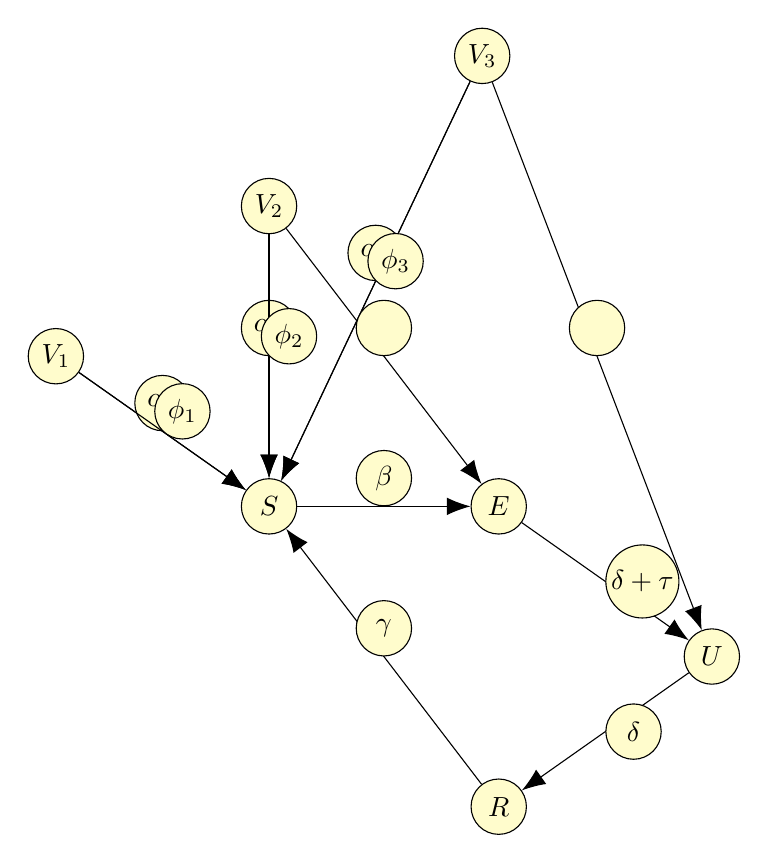
\begin{tikzpicture}[
node distance = 14mm and 22mm,
   box/.style = {circle, draw, fill=yellow!20, minimum size=2em, inner sep=1pt},
every node/.style = {box}
                    ]
\node (S)                               {$S$};
\node (V1) [above left=of S]            {$V_1$};
\node (V2) [above right=of V1]          {$V_2$};
\node (V3) [above right=of V2]          {$V_3$};
\node (E)  [right=of S]                 {$E$};
\node (U)  [below right=of E]           {$U$};
\node (R)  [below left=of U]            {$R$};

\draw[-{Latex[length=3mm]}] (V1) -- node [above] {$\alpha_1$} (S);
\draw[-{Latex[length=3mm]}] (S) -- node [above] {$\beta$} (E);
\draw[-{Latex[length=3mm]}] (E) -- node [right] {$\delta+\tau$} (U);
\draw[-{Latex[length=3mm]}] (U) -- node [right] {$\delta$} (R);
\draw[-{Latex[length=3mm]}] (R) -- node [above] {$\gamma$} (S);
\draw[-{Latex[length=3mm]}] (V2) -- node [above] {$\alpha_2$} (S);
\draw[-{Latex[length=3mm]}] (V3) -- node [above] {$\alpha_3$} (S);
\draw[-{Latex[length=3mm]}] (V1) -- node [above right] {$\phi_1$} (S);
\draw[-{Latex[length=3mm]}] (V2) -- node [above right] {$\phi_2$} (S);
\draw[-{Latex[length=3mm]}] (V3) -- node [above right] {$\phi_3$} (S);
\draw[-{Latex[length=3mm]}] (V2) -- node [above] {}(E); % Indicating a wait of 28 days is not shown as an edge but by context
\draw[-{Latex[length=3mm]}] (V3) -- node [above] {}(U); % Indicating a wait of 180 days is not shown as an edge but by context
\end{tikzpicture}

\end{document}